\documentclass[12pt]{article}

\usepackage{graphicx}
\graphicspath{ {./images/} }
\usepackage{paralist}
\usepackage{amsfonts}
\usepackage{amsmath}
\usepackage{hhline}
\usepackage{booktabs}
\usepackage{multirow}
\usepackage{multicol}
\usepackage{url}
\usepackage{hyperref}

\oddsidemargin -10mm
\evensidemargin -10mm
\textwidth 160mm
\textheight 200mm
\renewcommand\baselinestretch{1.0}

\pagestyle {plain}
\pagenumbering{arabic}

\newcounter{stepnum}

%% Comments

\usepackage{color}

\newif\ifcomments\commentstrue

\ifcomments
\newcommand{\authornote}[3]{\textcolor{#1}{[#3 ---#2]}}
\newcommand{\todo}[1]{\textcolor{red}{[TODO: #1]}}
\else
\newcommand{\authornote}[3]{}
\newcommand{\todo}[1]{}
\fi

\newcommand{\wss}[1]{\authornote{blue}{SS}{#1}}
\newcommand{\concat}{$\vert\vert$}

\title{Assignment 4, Specification}
\author{Mark Hutchison, COMP SCI 2ME3}

\begin{document}
\maketitle

The following specification is for the online game 2048. An online version of 2048 can be found at:

~\newline \href {https://play2048.co/} {https://play2048.co/} ~\newline

The version we will be implementing will be slightly different, but will follow the majority of the practices found in that game.

The game 2048 is a square matrix, refereed to as a board, of tiles. These tiles can slide from one end of the board to the opposite end, and perform ``merges'' while sliding when appropriate. A tile can ``merge'' with an empty tile as many times as it likes during a slide, but may only ``merge'' once with a tile of the same value during a slide.

The game ends when a user is incapable of performing any further ``merges'' in any direction available on a directional pad containing ``up'', ``down'', ``left'', and ``right''. For future reference, the directional pad referenced above will be dubbed the ``DPad'' for convince.

In some variants of 2048, the game may end when the user gets a tile on the board with the value of 2048. We will not be implementing this behavior. The game should be able to go on as long as possible in my opinion. Once the game is over, the user must be allowed to play again if they so choose. Also, if they reached a tile with 2048 as its value, they should be congratulated in some way, shape, or form when the game ends.

I accounted for change in this design by making everything as modular as possible, with as many freedoms that I could allow without ruining the specification.

\begin{itemize}
  \item Dividing the labour amongst the classes appropriately.
        \begin{itemize}
          \item The TileT stores the individual data of each TileT, such as value and colour.
          \item The BoardT handles the manipulation of said TileT's.
          \item The GameController interacts with the board to play the game, and stores things like score and highest TileT.
          \item The User then interacts with some sort of GUI to log their key inputs and play the game.
        \end{itemize}
  \item Allowing the game dimension, while being greater than 3, to be changed to allow the game to have variations that are more fun.
  \item Programming game mechanics to be modular within themselves, so changes can be done with only minor modifications. If something can be given a variable, it has been to allow the game to feel more customized to the user's preference without major modifications.
\end{itemize}

The View-Model-Controller pattern is also in itself a design for change, as it divides the 3 main concerns for further easy editing.

\begin{itemize}
  \item View: \texttt{GUIGraphics}
  \item Controller: \texttt{GameController}
  \item Model: \texttt{DirectionT}, \texttt{TileT}, \texttt{BoardT}
\end{itemize}

The final file structure is detailed roughly by this UML diagram:

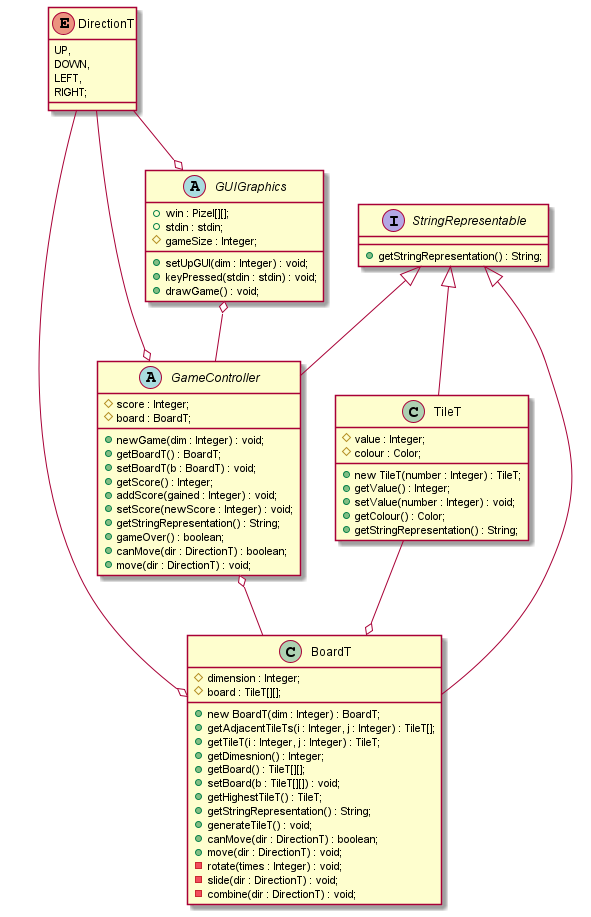
\includegraphics[width=4.5in]{2048_UML.png}

\newpage

\section* {DirectionT Module}

\subsection*{Module}

DirectionT

\subsection* {Uses}

None

\subsection* {Syntax}

\subsubsection* {Exported Constants}

None

\subsubsection* {Exported Types}

DirectionT = \{\\
UP, \\
DOWN, \\
LEFT, \\
RIGHT\\
\}

\subsubsection* {Exported Access Programs}

None

\subsection* {Semantics}

\subsubsection* {State Variables}

None

\subsubsection* {State Invariant}

None

\subsubsection* {Assumptions}

The only inputs available to the 2048 game are the 4 directions on a typical DPad.

\subsubsection* {Considerations}

When implementing in Java, use enums to define this like in Assignment 3 and Tutorial 7.

\newpage

\section* {StringRepresentable Interface Module}

\subsection* {Interface Module}

StringRepresentable

\subsection*{Uses}

None

\subsection* {Syntax}

\subsection*{Exported Constants}

None

\subsection*{Exported Types}

None

\subsubsection* {Exported Access Programs}

\begin{tabular}{| l | l | l | p{6cm} |}
  \hline
  \textbf{Routine name}   & \textbf{In} & \textbf{Out} & \textbf{Exceptions} \\
  \hline
  getStringRepresentation &             & $String$     &                     \\
  \hline
\end{tabular}

\newpage

\section* {TileT Module}

\subsection*{TileT Module inherits StringRepresentable}

TileT

\subsection* {Uses}

StringRepresentable

\subsection* {Syntax}

\subsubsection* {Exported Constants}

None

\subsubsection* {Exported Types}

TileT = ?

\subsubsection* {Exported Access Programs}

\begin{tabular}{| l | l | l | p{5cm} |}
  \hline
  \textbf{Routine name} & \textbf{In}  & \textbf{Out} & \textbf{Exceptions}      \\
  \hline
  new TileT             & $\mathbb{Z}$ & TileT        & IllegalArgumentException \\
  \hline
  getValue              &              & $\mathbb{Z}$ &                          \\
  \hline
  setValue              & $\mathbb{Z}$ &              & IllegalArgumentException \\
  \hline
  getColor              &              & $Color$      &                          \\
  \hline
\end{tabular}

\subsection* {Semantics}

\subsubsection* {State Variables}

$\mathit{value}: \mathbb{Z}$\\
$\mathit{c}$: $Color$

\subsubsection* {State Invariant}

$value > 0$

\subsubsection* {Assumptions}

$String(v: \mathbb{Z})$ returns a string containing the integer value of v.

\subsubsection* {Access Routine Semantics}

\noindent new TileT($number: \mathbb{Z}$):
\begin{itemize}
  \item transition: $value := number$
  \item output: $out := \mathit{self}$
  \item exception: $(number < 0) \Rightarrow IllegalArgumentException$
\end{itemize}

\noindent getTile():
\begin{itemize}
  \item output: $out := value$
  \item exception: None
\end{itemize}

\noindent setTile($number: \mathbb{Z}$):
\begin{itemize}
  \item output: $out := number$
  \item exception: $(number < 0) \Rightarrow IllegalArgumentException$
\end{itemize}

\noindent getColor():
\begin{itemize}
  \item output:

        \begin{tabular}{| p{3cm} | p{5cm} |}
          \hline
          Case         & out                  \\
          \hline
          value = 0    & Color(128, 128, 128) \\
          \hline
          value = 2    & Color(238, 228, 218) \\
          \hline
          value = 4    & Color(237, 224, 200) \\
          \hline
          value = 8    & Color(242, 177, 121) \\
          \hline
          value = 16   & Color(245, 149, 99)  \\
          \hline
          value = 32   & Color(246, 124, 95)  \\
          \hline
          value = 64   & Color(246, 94, 59)   \\
          \hline
          value = 128  & Color(237, 207, 114) \\
          \hline
          value = 256  & Color(237, 204, 97)  \\
          \hline
          value = 512  & Color(237, 200, 80)  \\
          \hline
          value = 1024 & Color(237, 197, 63)  \\
          \hline
          True         & Color(237, 194, 46)  \\
          \hline
        \end{tabular}
  \item exception: None
\end{itemize}

\noindent getStringRepresentation():
\begin{itemize}
  \item output: $out := String(value)$
  \item exception: None
\end{itemize}

\subsubsection{Considerations}

Implementation of \texttt{Color} is facilitated by the java \texttt{Color} class.

Color is custom type, represented as $tuple(\mathbb{Z}, \mathbb{Z}, \mathbb{Z})$, where the integers correspond to $(r, g, b)$.

\newpage

\section* {BoardT Module}

\subsection*{BoardT Module inherits StringRepresentable}

BoardT

\subsection* {Uses}

StringRepresentable, DirectionT, TileT

\subsection* {Syntax}

\subsubsection* {Exported Constants}

None

\subsubsection* {Exported Types}

BoardT = ?

\subsubsection* {Exported Access Programs}

\begin{tabular}{| l | l | l | l |}
  \hline
  \textbf{Routine name} & \textbf{In}                            & \textbf{Out}                           & \textbf{Exceptions}        \\
  \hline
  new BoardT            & $\mathbb{Z}$                           & BoardT                                 & IllegalArgumentException   \\
  \hline
  getDimension          &                                        & $\mathbb{Z}$                           &                            \\
  \hline
  getBoard              &                                        & $\text{seq [N] of (seq [N] of TileT)}$ &                            \\
  \hline
  setBoardT             & $\text{seq [N] of (seq [N] of TileT)}$ &                                        & IllegalArgumentException   \\
  \hline
  getTileT              & $\mathbb{Z}$, $\mathbb{Z}$             & $TileT$                                & IllegalArgumentException   \\
  \hline
  getAdjacentTileTs     & $\mathbb{Z}$, $\mathbb{Z}$             & $seq\ [4]\ of\ TileT$                  & IllegalArgumentException   \\
  \hline
  getHighestTileT       &                                        & $TileT$                                &                            \\
  \hline
  generateTileT         &                                        &                                        &                            \\
  \hline
  canMove               & $DirectionT$                           & $\mathbb{B}$                           &                            \\
  \hline
  move                  & $DirectionT$                           &                                        &                            \\
  \hline
\end{tabular}

\subsection* {Semantics}

\subsubsection* {State Variables}

$\mathit{dimension}$: $\mathbb{Z}$\\
$\mathit{board}: \text{seq [dimension] of (seq [dimension] of TileT)}$\\

\subsubsection* {State Invariant}

$dimension > 0$

\subsubsection* {Assumptions}

None

\subsubsection* {Access Routine Semantics}

\noindent new BoardT($dim: \mathbb{Z}$):
\begin{itemize}
  \item transition: $dimension, board := dim, \langle i: \mathbb{N}\ \vert\ 0 < i < dimension: \langle j: \mathbb{N}\ \vert\ 0 < j < dimension: \text{ new TileT(0)}\rangle\rangle$
  \item output: $out := \mathit{self}$
  \item exception: $(dim < 3) \Rightarrow IllegalArgumentException$
\end{itemize}

\noindent getBoard():
\begin{itemize}
  \item output: $out := board$
  \item exception: None
\end{itemize}

\noindent getDimension():
\begin{itemize}
  \item output: $out := dimension$
  \item exception: None
\end{itemize}

\noindent setBoard($b: \text{seq [N] of (seq [N] of TileT)}$):
\begin{itemize}
  \item transition: $board, dimension := b, N$
  \item exception: $\lnot (N < 3) \Rightarrow IllegalArgumentException$
  \item assumption: board is a square matrix of TileTs, and $N: \mathbb{N}$
\end{itemize}

\noindent getTileT($i: \mathbb{Z}, j: \mathbb{Z}$):
\begin{itemize}
  \item output: $out := board$
  \item exception: $\lnot (0 \le i, j < dimension) \Rightarrow IllegalArgumentException$
\end{itemize}

\noindent getAdjacentTileTs($i: \mathbb{Z}, j: \mathbb{Z}$):
\begin{itemize}
  \item output: $out := \langle\text{up, down, left, right}\rangle$ where:
        \begin{flalign*}
          up    & := \lnot (0 \le i - 1 < dimension) \Rightarrow NIL\ \vert\ True \Rightarrow board[i-1][j] & \\
          down  & := \lnot (0 \le i + 1 < dimension) \Rightarrow NIL\ \vert\ True \Rightarrow board[i+1][j] & \\
          left  & := \lnot (0 \le j - 1 < dimension) \Rightarrow NIL\ \vert\ True \Rightarrow board[i][j-1] & \\
          right & := \lnot (0 \le j + 1 < dimension) \Rightarrow NIL\ \vert\ True \Rightarrow board[i][j+1] & \\
        \end{flalign*}
  \item exception: $\lnot (0 < i, j < dimension) \Rightarrow IllegalArgumentException$
\end{itemize}

\noindent getHighestTileTs():
\begin{itemize}
  \item output: $out := max(\langle i \in \mathbb{N} . (i < dimesnion) \Rightarrow maxValue(board[i]) \rangle)$

        See local functions for implementation details of $maxValue()$
  \item exception: None
  \item assumptions: max is a defined function that simply returns the largest integer in a sequence of integers.
\end{itemize}

\noindent generateTileT():
\begin{itemize}
  \item transition:

        \begin{tabular}{|l|l|l|}
          \hline
                                                          &                                        & $board[i][j] :=$      \\
          \hline
          \multirow{2}{*}{$getTileT(i,j).getValue() = 0$} & $random(0, 10) < 2$                    & $\text{new TileT(4)}$ \\
          \cline{2-3}
                                                          & True                                   & $\text{new TileT(2)}$ \\
          \hline
          $getTileT(i,j).getValue() \ne 0$                & \multicolumn{2}{c|}{$generateTileT()$}                         \\
          \hline
        \end{tabular}

        where: \\
        $i := random(0 ,dimension - 1)$ \\
        $j := random(0 ,dimension - 1)$

  \item assumptions: The function $random(a: \mathbb{N}, b: \mathbb{N})$ described returns an integer in between $a$ and $b$ inclusive. Additionally, this function will only be called when there is a spot available for the TileT to be inserted.
\end{itemize}

\noindent canMove($dir: DirectionT$):
\begin{itemize}
  \item out: $out := \exists(i,j:\mathbb{N}\ \vert 0 < i,j < dimension:$

        \noindent\begin{flalign*}
          dir.equals(DirectionT.UP)    & \Rightarrow (getAdjacentTileTs(i,j)[0].getValue() = 0                        \\
                                       & \vee getAdjacentTileTs(i,j)[0].getValue() = getTileT(i,j).getValue())\ \vert \\
          dir.equals(DirectionT.DOWN)  & \Rightarrow (getAdjacentTileTs(i,j)[1].getValue() = 0                        \\
                                       & \vee getAdjacentTileTs(i,j)[1].getValue() = getTileT(i,j).getValue())\ \vert \\
          dir.equals(DirectionT.LEFT)  & \Rightarrow (getAdjacentTileTs(i,j)[2].getValue() = 0                        \\
                                       & \vee getAdjacentTileTs(i,j)[2].getValue() = getTileT(i,j).getValue())\ \vert \\
          dir.equals(DirectionT.RIGHT) & \Rightarrow (getAdjacentTileTs(i,j)[3].getValue() = 0                        \\
                                       & \vee getAdjacentTileTs(i,j)[3].getValue() = getTileT(i,j).getValue())        \\
          )
        \end{flalign*}
  \item exception: None
\end{itemize}

\noindent move($dir: DirectionT$):
\begin{itemize}
  \item transition: \\
        \begin{tabular}{|l|p{5cm}|}
          \hline
                                                          & instructions \\
          \hline
          \multirow{5}{*}{$dir.equals(DirectionT.UP)$}    & $rotate(3)$  \\
                                                          & $slide()$    \\
                                                          & $combine()$  \\
                                                          & $slide()$    \\
                                                          & $rotate(1)$  \\
          \hline
          \multirow{5}{*}{$dir.equals(DirectionT.DOWN)$}  & $rotate(1)$  \\
                                                          & $slide()$    \\
                                                          & $combine()$  \\
                                                          & $slide()$    \\
                                                          & $rotate(3)$  \\
          \hline
          \multirow{5}{*}{$dir.equals(DirectionT.LEFT)$}  & $rotate(2)$  \\
                                                          & $slide()$    \\
                                                          & $combine()$  \\
                                                          & $slide()$    \\
                                                          & $rotate(2)$  \\
          \hline
          \multirow{3}{*}{$dir.equals(DirectionT.RIGHT)$} & $slide()$    \\
                                                          & $combine()$  \\
                                                          & $slide()$    \\
          \hline
        \end{tabular}

        See local functions for specifications regarding functions used.
  \item exception: None
\end{itemize}

\noindent getStringRepresentation():
\begin{itemize}
  \item output:
        \noindent The string representation of a board is quite an involved process, and is hard to write mathematically. The returned value of this method is a string representation of the game board using design characters. The process of generating this string is broken into steps:

        \begin{enumerate}
          \item Define $tileLength$ as

                $min(6,\ 2 + \vert\vert\text{gameController.getHighestTile().getStringRepresentation()}\vert\vert)$

          \item Now we need to pick our Decoration Alphabet for the board. Your alphabet, at minimum, will include:

                \begin{itemize}
                  \item 4 corner characters: denoted as $TL$, $TR$, $BL$, $BR$
                  \item A horizontal line character: denoted as $-$
                  \item A vertical line character: denoted as $l$
                  \item At minimum 1 ``join'' character: denoted as $+$
                  \item A Blank Space character: denoted as $BS$
                  \item A newline character: denoted as LF.
                \end{itemize}

          \item The final tools we will need are two operators, concatenate (\concat) and repeat ($*$)

          \item We first set
                $out := $ ``$TL$ \concat ($(- * tileLength)$ \concat $+$) $* dimension - 1$ \concat ($(- * tileLength)$) \concat $TR$ \concat $LF$''

          \item Now we need to preform two iterations of code, one that occurs for every $arr:\ seq\ [dimension]\ of\ TileT \in board$, and one for every $t:\ TileT \in arr$.

                \begin{enumerate}
                  \item For every $arr$, we concatenate a ``$l$'' character to the string.

                  \item Then for every $t:\ TileT \in arr$, if $t.getValue() > 0$,

                        $out := outs$ \concat ``$BS * (tileLength - \lfloor\frac{tileLength}{2}\rfloor)$ \concat $t.getStringRepresentation()$ \concat $BS * (tileLength - \lceil\frac{tileLength}{2}\rceil)$ \concat $l$'',

                        Else,

                        $out :=$ \concat ``$BS * tileLength$ \concat $l$''

                  \item If $arr$ is not the last sequence found in $board$,
                        $out := out$ \concat ``$LF$ \concat $+$ \concat (($- * tileLength$) \concat $+$) $* dimension - 1$ \concat $(- * tileLength)$ \concat $+$ \concat $LF$''
                        Else, just $out := out$ \concat ``LF''
                \end{enumerate}

          \item Finally, we conclude our string:

                $out := out$ \concat ``$BL$ \concat ($-$ $* tileLength$ \concat $+$) $* dimension - 1$ \concat ($- * tileLength$) \concat $BR$ \concat $LF$''
        \end{enumerate}

        The method described above should render a complete ASCII board representation of the data in $board$.

  \item exception: None
\end{itemize}

\subsubsection* {Local Routines}

\noindent maxValue($row:\ seq\ [dimension]\ of\ TileT$):
\begin{itemize}
  \item output: $out := max(\langle i \in \mathbb{N}\ .\ (i < dimesnion) \Rightarrow row[i].getValue() \rangle)$
  \item exception: None
  \item assumptions: max is a defined function that simply returns the largest integer in a sequence of integers.
\end{itemize}

\noindent rotate($n:\ \mathbb{Z}$):
\begin{itemize}
  \item transition: \\
        \noindent For every k: $\mathbb{N}$ where $0 \le k < n$:                                                         \\
        \noindent\hspace*{0.5cm} For every i: $\mathbb{N}$ where $0 \le i < dimension$:                                  \\
        \noindent\hspace*{1cm} For every j: $\mathbb{N}$ where $i \le j < dimension$:                                    \\
        \noindent\hspace*{1.5cm} $board[i][j], board[j][i] := board[j][i], board[i][j]$                                  \\
        \noindent\hspace*{0.5cm}For every i: $\mathbb{N}$ where $0 \le i < dimension$:                                   \\
        \noindent\hspace*{1cm} For every j: $\mathbb{N}$ where $i \le j < \lfloor \frac{dimension}{2} \rfloor$:          \\
        \noindent\hspace*{1.5cm} $board[i][j],  board[i][dimension - 1 - j] := board[i][dimension - 1 - j], board[i][j]$
  \item exception: None
\end{itemize}

\noindent slide():
\begin{itemize}
  \item transition:\\
        \noindent For every k: $\mathbb{N}$ where $0 \le i < dimension$: \\
        \noindent\hspace*{0.5cm} For every i: $\mathbb{N}$ where $dimension - 1 > i \ge 0$: \\
        \noindent\hspace*{1cm} For every j: $\mathbb{N}$ where $i \le j < dimension$: \\
        \noindent\hspace*{1.5cm} $(board[k][j].getValue() \ne 0 \wedge board[k][j + 1].getValue() = 0) \Rightarrow board[k][j], board[k][j+1] := board[k][j+1], board[k][j]$
  \item exception: None
\end{itemize}

\noindent combine():
\begin{itemize}
  \item transition:\\
        \noindent For every k: $\mathbb{N}$ where $0 \le i < dimension$: \\
        \noindent\hspace*{0.5cm} For every i: $\mathbb{N}$ where $dimension - 1 \ge i > 0$: \\
        \noindent\hspace*{1.45cm} $(board[k][i].getValue() \ne 0 \wedge board[k][i].getValue() = board[k][i - 1].getValue()) \Rightarrow$\\
        \noindent\hspace*{1.45cm} $\{$\\
        \noindent\hspace*{1.95cm} $GameController.addScore(board[k][i - 1].getValue() * 2);$\\
        \noindent\hspace*{1.95cm} $board[k][i] := new TileT(board[k][i - 1].getValue() * 2);$\\
        \noindent\hspace*{1.95cm} $board[k][i - 1] := new TileT();$\\
        \noindent\hspace*{1.45cm} $\}$
  \item exception: None
\end{itemize}

\newpage

\section* {GameController Module (Abstract Object)}

\subsection*{GameController Module inherits StringRepresentable}

GameController

\subsection* {Uses}

StringRepresentable, DirectionT, TileT, BoardT

\subsection* {Syntax}

\subsubsection* {Exported Constants}

None

\subsubsection* {Exported Types}

GameController = ?

\subsubsection* {Exported Access Programs}

\begin{tabular}{| l | l | l | p{5cm} |}
  \hline
  \textbf{Routine name} & \textbf{In}  & \textbf{Out} & \textbf{Exceptions}        \\
  \hline
  newGame               & $\mathbb{Z}$ &              &                            \\
  \hline
  getBoard              &              & $BoardT$     & IllegalArgumentException \\
  \hline
  setBoard              & $BoardT$     &              &                            \\
  \hline
  getScore              &              & $\mathbb{Z}$ &                            \\
  \hline
  addScore              & $\mathbb{Z}$ &              &                            \\
  \hline
  setScore              & $\mathbb{Z}$ &              &                            \\
  \hline
  gameOver              &              & $\mathbb{B}$ &                            \\
  \hline
  canMove               & $DirectionT$ & $\mathbb{B}$ &                            \\
  \hline
  move                  &              &              &                            \\
  \hline
\end{tabular}

\subsection* {Semantics}

\subsubsection* {State Variables}

$\mathit{score}: \mathbb{Z}$\\
$\mathit{board}$: $BoardT$

\subsubsection* {State Invariant}

$score \ge 0$

\subsubsection* {Assumptions}

None

\subsubsection* {Access Routine Semantics}

\noindent newGame($dim: \mathbb{Z}$):
\begin{itemize}
  \item transition: $board, score := new BoardT(dim), 0$
  \item exception: $dim >= 3 \Rightarrow IllegalArgumentException$
\end{itemize}

\noindent getBoardT():
\begin{itemize}
  \item out: $out := board$
  \item exception: None
\end{itemize}

\noindent setBoardT($b: BoardT$):
\begin{itemize}
  \item transition: $board := b$
  \item exception: None
\end{itemize}

\noindent getScore():
\begin{itemize}
  \item out: $out := score$
  \item exception: None
\end{itemize}

\noindent addScore($num: \mathbb{N}$):
\begin{itemize}
  \item transition: $score := score + num$
  \item exception: None
\end{itemize}

\noindent setScore($num: \mathbb{N}$):
\begin{itemize}
  \item transition: $score := num$
  \item exception: None
\end{itemize}

\noindent canMove($dir: DirectionT$):
\begin{itemize}
  \item out: $out := board.canMove(dir)$
  \item exception: None
\end{itemize}

\noindent move($dir: DirectionT$):
\begin{itemize}
  \item transition: $board := board.move(dir); board.generateTileT()$
  \item exception: None
\end{itemize}

\noindent gameOver():
\begin{itemize}
  \item out: $out := True$\hfill\\
        \noindent For every i: $\mathbb{N}$ where $0 \le i < board.getDimension()$: \\
        \noindent\hspace*{0.5cm} For every j: $\mathbb{N}$ where $0 \le i < board.getDimension()$: \\
        \noindent\hspace*{1cm} $(board.getTileT(i,j).getValue() = 0) \Rightarrow\ out:= False$ \\
        \noindent\hspace*{1cm} For every $tile: TileT \in board.getAdjacentTileTs(i, j)$: \\
        \noindent\hspace*{1.5cm} $(board.getTileT(i, j).getValue() = tile.getValue()) \Rightarrow\ out:= False$
  \item description: This function will return the final result of $out$ after preforming the operations described. $out$ is by default $True$, and becomes $False$ when a condition violates the gameOver condition.
  \item exception: None
\end{itemize}

\noindent getStringRepresentation():
\begin{itemize}
  \item output: $out := $ ``2048 \concat LF \concat $board.getStringRepresentation()$ \concat LF \concat  Score: \concat $score$ \concat LF \concat Highest Tile: \concat LF \concat $board.getHighestTileT().getValue().getStringRepresentation()$''\\

        $out := (board.getHighestTileT().getValue() = 2048) \Rightarrow out$ \concat ``Congratulations! \concat LF \concat Press 'Enter' to Restart or Keep Playing! \concat LF'' $\vert $\\

        $True \Rightarrow out$ \concat ``Press 'Enter' to Start! \concat LF \concat Press 'wasd' or Arrow Keys to slide! \concat LF''
  \item exception: None
\end{itemize}

\newpage

\newpage

\section* {GUIGraphics Module}

\subsection* {Module}

GUIGraphics

\subsection* {Uses}

None

\subsection* {Syntax}

\subsubsection* {Exported Constants}

None

\subsubsection* {Exported Access Programs}

\begin{tabular}{| l | l | l | l |}
  \hline
  \textbf{Routine name} & \textbf{In}  & \textbf{Out} & \textbf{Exceptions}        \\
  \hline
  $setUpGUI$            & $\mathbb{N}$ &              & IllegalArgumentException \\
  \hline
  $keyPressed$          & $stdin$      &              &                            \\
  \hline
  $drawGame$            &              &              &                            \\
  \hline
\end{tabular}

\subsection* {Semantics}

\subsubsection* {Environment Variables}

win: two dimensional sequence of coloured pixels

\noindent stdin: the standard input used by the user, like a keyboard

\subsubsection* {State Variables}

$\mathit{gameSize}: \mathbb{N}$

\subsubsection* {State Invariant}

$gameSize >= 3$

\subsubsection* {Assumptions}

stdin will, at minimum, contain one set of inputs that clearly and explicitly translates to the standard DPad directions.

The GUI will be designed for a 4x4 game board, but should be able to render larger even if not athletically pleasing.

\subsubsection* {Access Routine Semantics}

\noindent setUpGUI($dim: \mathbb{N}$):
\begin{itemize}
  \item transition: $GameController.newGame(dim); gameSize := dim$

        After the game controller is set up, preform the necessary steps to set up a game window on $win$, and populate it with the appropriate information. For the information you should render, refer to $GameController.getStringRepresentation()$.

        After this setup, call $drawGame$.

  \item exception: $dim < 3 \Rightarrow IllegalArgumentException$
\end{itemize}

\noindent keyPressed():
\begin{itemize}
  \item transition: Monitor $stdin$ for the user pressing any valid DPad direction or the starting key of your choice. Upon pressing the starting key, preform the following:
        \begin{flalign*}
           & GameController.newGame(gameSize)           \\
           & GameController.getBoardT().generateTileT() \\
           & GameController.getBoardT().generateTileT()
        \end{flalign*}

        Upon pressing any DPad key, find the $dir: DirectionT$ that matches it, and preform the following $GameController.canMove(dir) \Rightarrow GameController.move(dir)$

  \item exception: None
\end{itemize}

\noindent drawGamer():
\begin{itemize}
  \item transition:

        Simply render the game state to $win$, referring to $GameController.getStringRepresentation()$ for items that need to be rendered.

        Every transition of the GameController's board state should re-render the game board using this routine.

  \item exception: None
\end{itemize}

\subsubsection{Considerations}

Implementation of \texttt{GUIGraphics.java} is facilitated by the java \texttt{swing} library.

\newpage

\section* {Critique of my Design}

The critique of a design comes down to 4 properties:

\begin{itemize}
  \item Consistent: I did everything in my power to remain consistent in this specification. I used Camel Case whenever possible, I kept variable names similar, and it is all done in my writing style (good or bad as that may be). I did everything in my power to maintain a level of consistency and opacity when it came to writing this specification.
  \item Essential: Essential means that no two routines in the same module do the same thing, and I can say with confidence that this is true. However, I wanted to point out a place of worry: The gameController does contain routines that do nothing but call the routine of the game BoardT and propagates the value. This is still technically essential, and is the point of the design patter, but it is still a place that I think needs to be discussed when talking about essential design.
  \item Minimal: I kept my Model as minimal as possible, however I sacrificed this quality when finishing my \texttt{BoardT} and coding my \texttt{GameController}. For example, \texttt{GameController.move()} both moves the board, but also generates a \texttt{TileT} at the same time. It makes sense to combine these into one, but it isn't minimal.
  \item Generality: This is very literal sadly, and not very general. Looking at the specification, there is only 1 use case for every type and it is extremely explicit in the use case. I didn't even try to make this general, as that is time I couldn't spend due to the amount of work.
\end{itemize}

\end{document}